\documentclass[conference]{IEEEtran}

%% DOCUMENT FORMATTING
\usepackage[ngerman]{babel}
\usepackage{csquotes}
\usepackage{geometry}

%% Hyperlinks
\usepackage{hyperref}

%% GRAPHICS
\usepackage{graphicx}

% CITATION
\usepackage{acronym}

\usepackage[style=ieee, maxcitenames=2, mincitenames=1]{biblatex}
\addbibresource{sources.bib}


\def\BibTeX{{\rm B\kern-.05em{\sc i\kern-.025em b}\kern-.08em
    T\kern-.1667em\lower.7ex\hbox{E}\kern-.125emX}}
\begin{document}
\pagenumbering{Roman} 

\title{Generatives KI-Design\\
\large \ \\ \large Wie beeinflusst generatives Design die kreativen Gestaltungsprozesse in der Designbranche?}

\author{
  \IEEEauthorblockN{Alexandros Loukaridis}
  \IEEEauthorblockA{\textit{MatNr. 1000730} \\
  92loal1bif@hft-stuttgart.de}

  \and

  \IEEEauthorblockN{Valentin Franco}
  \IEEEauthorblockA{\textit{MatNr. 380094} \\
  91frva1bif@hft-stuttgart.de}
}

\maketitle

\begin{abstract}

    Diese Seminararbeit untersucht den Einfluss des Generativen Designs auf kreative Gestaltungsprozesse in der Designbranche. Die zentrale Fragestellung lautet: Wie beeinflusst das Generative Design den Entscheidungsprozess und die kreative Intuition der Designer? Um diese Frage zu beantworten, werden verschiedene Methoden des Generativen Designs untersucht, darunter parametrisches Design, algorithmisches Design, evolutionäre Algorithmen, prozedurale Generierung, Simulation und Analyse, Machine Learning und Künstliche Intelligenz, generative Algorithmen sowie datengesteuertes Design.
    
    Im Rahmen dieser Seminararbeit werden die grundlegenden Konzepte und Eigenschaften des Generativen Designs erläutert. Dabei liegt der Fokus auf mathematischen Modellen, Regelsystemen und Algorithmen, die zur Beschreibung und Manipulation von formalen und ästhetischen Eigenschaften von Designs verwendet werden. Es werden Fallbeispiele und Anwendungen des Generativen Designs in verschiedenen Bereichen wie Architektur, Produktgestaltung, Grafikdesign, Kunst, Modedesign, Industriedesign sowie Medizin und Gesundheitswesen untersucht.
    
    Die Ergebnisse dieser Untersuchung zeigen, dass das Generative Design einen signifikanten Einfluss auf die kreativen Gestaltungsprozesse hat. Es ermöglicht Designern, effizienter zu arbeiten, Materialersparnisse zu erzielen und innovative Lösungen zu generieren. Durch die Integration von automatisierten Prozessen und algorithmischen Methoden eröffnet das Generative Design neue Wege der Gestaltung, die über traditionelle Designansätze hinausgehen.
    
    Die Folgerungen aus dieser Seminararbeit sind vielfältig. Das Generative Design bietet Potenziale für eine effizientere Gestaltung, die Reduzierung des Materialverbrauchs, die Förderung von Innovationen und eine hohe Anpassungsfähigkeit. Es ermöglicht es Designern, verschiedene Variationen und Optionen zu erkunden und maßgeschneiderte Lösungen für unterschiedliche Nutzerbedürfnisse zu entwickeln. Die Erkenntnisse dieser Arbeit haben Implikationen für die Designpraxis und bieten Anwendungsmöglichkeiten in verschiedenen Bereichen.
    
    Insgesamt liefert diese Seminararbeit ein umfassendes Verständnis für das Generative Design und seine Auswirkungen auf die Designbranche. Sie bietet eine Grundlage für die Diskussion über die Zukunft der kreativen Gestaltungsprozesse und zeigt Wege auf, wie das Generative Design in der Praxis angewendet werden kann, um innovative Lösungen zu generieren.

\end{abstract}

\section{Einleitung}
Generatives Design mit künstlicher Intelligenz hat in den letzten Jahren einen großen Einfluss auf das Produktdesign und 
die Fertigung von Produkten gewonnen. Es ermöglicht Unternehmen, innovative und maßgeschneiderte Lösungen für ihre Kunden 
zu schaffen, indem es automatisiert verschiedene Designoptionen generiert und optimiert. Dabei wird ein Satz von Parametern 
und Kriterien definiert, die das Design beeinflussen, und dann werden unzählige Design-Optionen von der KI generiert, die die 
Vorgaben erfüllen. Anschließend können die besten Optionen ausgewählt werden, um das endgültige Produkt zu entwickeln.
Dieser Prozess bietet eine effiziente Möglichkeit, die Effektivität und Leistung von Produkten zu verbessern und gleichzeitig 
den Materialverbrauch und die Herstellungskosten zu reduzieren. Es hat sich gezeigt, dass Unternehmen, die generatives Design 
und künstliche Intelligenz nutzen, ihre Produkte schneller auf den Markt bringen können, wettbewerbsfähiger sind und bessere 
Kundenzufriedenheit erreichen.

Ein herausragendes Beispiel für den Einsatz von generativem Design mit künstlicher Intelligenz ist der Nike Flyprint-Schuh. 
Nike hat in Zusammenarbeit mit Autodesk das Design-Tool entwickelt, um den Schuh durch generatives Design zu entwerfen. Der 
Schuh wurde speziell für Athleten entwickelt und sollte eine optimale Passform und Leistung bieten. Durch die Verwendung von 
generativem Design mit künstlicher Intelligenz konnte Nike schnell und effizient tausende von Design-Optionen generieren und 
die besten Optionen für den Schuh auswählen. Das Ergebnis war ein innovativer Schuh, der den Anforderungen von Athleten gerecht
 wurde und gleichzeitig den Materialverbrauch reduzierte. 

Nike's Flyprint-Schuh, der durch generatives Design mit künstlicher Intelligenz entworfen wurde, ist nur ein Beispiel für die 
vielen Anwendungen von künstlicher Intelligenz im Produktdesign. Doch wie genau wird generatives Design mit künstlicher Intelligenz
eingesetzt und welche Auswirkungen hat es auf die Produktdesign-Branche?

\section{Grundlagen des generativen Designs}
\subsection*{Definition und Konzepte des Generativen Designs}
Generatives Design ist ein multidisziplinärer Ansatz, der Prinzipien aus Design, Informatik, Mathematik und Ingenieurwissenschaften kombiniert, um komplexe und innovative Lösungen zu entwickeln. Es basiert auf der Idee, dass ein Designprozess nicht nur von einem einzelnen Designer gesteuert wird, sondern dass algorithmische Systeme und computergestützte Generierungstechniken eingesetzt werden, um eine Vielzahl von Designoptionen zu erzeugen.

Bei generativem Design steht die Erstellung von Regeln, Parametern und Algorithmen im Vordergrund, die es ermöglichen, eine Vielzahl von Designvarianten automatisch zu generieren. Diese Varianten können auf bestimmten Designkriterien und Zielen basieren, die zuvor definiert wurden. Durch den Einsatz von Rechenleistung und automatisierter Generierung können komplexe Probleme analysiert und alternative Designlösungen entwickelt werden.

Das Konzept des generativen Designs basiert auf der Vorstellung, dass das Design nicht nur ein statisches Endprodukt ist, sondern ein iterativer und dynamischer Prozess, der verschiedene Entwurfsiterationen und Explorationen umfasst. Es ermöglicht eine systematische Untersuchung des Designraums, um optimale Lösungen zu finden und unkonventionelle Ansätze zu entdecken.

Ein weiteres wichtiges Konzept im generativen Design ist die Parameterisierung. Durch die Festlegung von Parametern können bestimmte Aspekte des Designs flexibel gesteuert und variiert werden. Dadurch können verschiedene Designvarianten erzeugt werden, indem die Parameterwerte verändert werden. Dies ermöglicht es, schnell verschiedene Designoptionen zu erkunden und alternative Lösungen zu generieren.

Das generative Design kann auch auf das Konzept der Emergenz zurückgeführt werden. Emergenz bezieht sich auf die Eigenschaften und Muster, die aufgrund der Interaktion und des Zusammenspiels von Elementen in einem System entstehen. Im generativen Design können emergente Eigenschaften in den generierten Designs auftreten, die nicht direkt von einem Designer vorhergesehen oder geplant wurden. Dies führt zu überraschenden und innovativen Lösungen.

Generatives Design wird in verschiedenen Bereichen eingesetzt, darunter Architektur, Produktdesign, Grafikdesign, Modedesign und viele andere. Es bietet die Möglichkeit, komplexe Gestaltungsprobleme anzugehen, effizientere Designs zu entwickeln, personalisierte Lösungen zu erstellen und innovative Ansätze zu fördern.
\subsection*{Historischer Überblick}
Der Ursprung des generativen Designs lässt sich bis in die 1960er Jahre zurückverfolgen, als sich die Informatik und die digitale Technologie zu entwickeln begannen. Zu dieser Zeit wurden erste Versuche unternommen, algorithmische Ansätze in den Designprozess einzuführen.

Ein bedeutendes Ereignis in der Geschichte des generativen Designs war die Gründung des Massachusetts Institute of Technology (MIT) Media Lab im Jahr 1985. Hier wurden bahnbrechende Forschungen im Bereich des computergestützten Designs durchgeführt, die die Grundlagen für das generative Design legten. Unter der Leitung von Designern wie John Maeda und William J. Mitchell wurden neue Methoden und Werkzeuge entwickelt, um computerbasierte Generierungstechniken in den Designprozess zu integrieren.

In den 1990er Jahren begannen sich parametrische Designsysteme zu etablieren. Eines der bekanntesten Beispiele ist das Programm "Generative Components", das von dem Architekten und Designer Cecil Balmond und seinem Team bei Arup entwickelt wurde. Diese Systeme ermöglichten es den Designern, Parameter und Regeln festzulegen, um Variationen von Designlösungen zu generieren und zu optimieren.

Ein weiterer Meilenstein in der Geschichte des generativen Designs war die Entwicklung von evolutionären Algorithmen. Der Informatiker Karl Sims pionierte in den 1990er Jahren die Verwendung von evolutionären Algorithmen zur Erzeugung von virtuellen Welten und künstlerischen Formen. Diese Algorithmen basieren auf Prinzipien der natürlichen Evolution und ermöglichen es, durch Variation, Selektion und Mutation Designs zu generieren und zu verbessern.

Mit dem Aufkommen leistungsstärkerer Computer und der Fortschritte in der Künstlichen Intelligenz (KI) und dem maschinellen Lernen eröffneten sich neue Möglichkeiten für das generative Design. Machine-Learning-Algorithmen können große Datenmengen analysieren und Muster erkennen, um Designs automatisch zu generieren. Diese Entwicklung hat zu einer verstärkten Integration von KI-Techniken in den Designprozess geführt und ermöglicht es Designern, neue Wege der Gestaltung zu erkunden.

Heutzutage hat das generative Design in verschiedenen Bereichen wie Architektur, Produktdesign, Grafikdesign, Modedesign und anderen an Bedeutung gewonnen. Es wird von Designern, Ingenieuren und Künstlern eingesetzt, um komplexe Probleme anzugehen, innovative Lösungen zu entwickeln und neue ästhetische Ausdrucksformen zu erkunden.

Der historische Überblick zeigt, dass das generative Design eng mit dem Fortschritt der digitalen Technologie und der Entwicklung neuer Designmethoden verbunden ist. Durch die Integration von algorithmischen Ansätzen, parametrischen Systemen, evolutionären Algorithmen und KI-Techniken hat sich das generative Design zu einem wichtigen Bereich im zeitgenössischen Design entwickelt, der die kreative Gestaltung maßgeblich beeinflusst.

\subsection*{Anwendungsgebiete des Generativen Designs}
Generatives Design findet in verschiedenen Branchen und Anwendungsgebieten Anwendung. Es ermöglicht die Lösung komplexer Gestaltungsprobleme, die Entwicklung innovativer Produkte und die Schaffung einzigartiger ästhetischer Ausdrucksformen. Auf die genauen Einsatzgebiete wird in Kapitel IV eingegangen.


\section{Methoden des Generativen Designs}

1. Parametrisches Design: Die Verwendung von parametrischen Modellen, bei denen Designelemente und -parameter miteinander verknüpft sind. Durch die Anpassung dieser Parameter können verschiedene Designvarianten generiert werden. Beispiel: Ein Architekt nutzt parametrisches Design, um automatisch verschiedene Variationen eines Gebäudes zu generieren, indem er Parameter wie Größe, Form und Material anpasst.

2. Algorithmisches Design: Die Anwendung von Algorithmen zur Generierung von Designs. Diese Algorithmen können Regeln, Bedingungen und Zufallselemente enthalten, um unterschiedliche Ergebnisse zu erzielen. Beispiel: Ein Grafikdesigner nutzt algorithmisches Design, um automatisch verschiedene Logo-Designs zu generieren, indem er Regeln und Variationen in Form, Farbe und Anordnung festlegt.

3. Evolutionäre Algorithmen: Die Anwendung von genetischen oder evolutionären Algorithmen, um Designs zu generieren und zu optimieren. Dabei werden Designvarianten erzeugt, bewertet und miteinander kombiniert, um immer bessere Ergebnisse zu erzielen. Beispiel: Ein Fahrzeughersteller verwendet evolutionäre Algorithmen, um verschiedene Fahrzeugdesigns zu generieren und sie basierend auf Kriterien wie Aerodynamik, Effizienz und Ästhetik zu optimieren.

4. Prozedurale Generierung: Die Nutzung von Regeln, Algorithmen oder Programmcode, um automatisch Designs zu erzeugen. Prozedurale Generierung ermöglicht die Erzeugung von komplexen und vielfältigen Designs, indem wiederholbare Verfahren angewendet werden. Beispiel: In der Videospielentwicklung wird prozedurale Generierung verwendet, um automatisch Landschaften, Levels und Charaktere zu erstellen, wodurch eine große Vielfalt an Spielinhalten generiert werden kann.

5. Simulation und Analyse: Die Verwendung von Simulationen und Analysewerkzeugen, um das Verhalten, die Leistung oder andere Aspekte des Designs zu bewerten. Dies ermöglicht eine iterative Optimierung und Verbesserung des Designs. Beispiel: Ein Architekt nutzt Simulationen, um den Energieverbrauch und die thermische Leistung eines Gebäudes zu analysieren und das Design entsprechend anzupassen, um eine optimale Energieeffizienz zu erreichen.

6. Machine Learning und Künstliche Intelligenz: Der Einsatz von maschinellen Lernverfahren und künstlicher Intelligenz, um aus vorhandenen Daten zu lernen und neue Designs zu generieren. Dabei können Muster, Stile oder Präferenzen aus einer Vielzahl von Beispielen erlernt werden. Beispiel: Ein Unternehmen für medizinische Geräteentwicklung nutzt maschinelles Lernen, um aus einer großen Menge von Patientendaten Designs für personalisierte medizinische Geräte zu generieren, die den individuellen Bedürfnissen und Präferenzen der Benutzer entsprechen.

7. Generative Algorithmen: Die Nutzung von spezifischen Algorithmen, die auf generativen Prinzipien basieren, um neue Designs zu erzeugen. Diese Algorithmen können auf Regeln, Wahrscheinlichkeiten oder emergentem Verhalten basieren. Beispiel: Ein Künstler verwendet generative Algorithmen, um abstrakte Kunstwerke zu generieren, indem er Regeln für Formen, Farben und Bewegungen festlegt, die zu einzigartigen und dynamischen Ergebnissen führen.

8. Datengesteuertes Design: Die Verwendung von Daten, um Designs zu generieren oder zu beeinflussen. Dies können beispielsweise Umgebungsdaten, Benutzerpräferenzen oder andere Informationen sein, die in den Generierungsprozess einfließen. Beispiel: Ein Webdesigner nutzt datengesteuertes Design, um die Benutzererfahrung zu verbessern, indem er das Design einer Website basierend auf dem Verhalten der Benutzer anpasst, um deren Bedürfnisse und Vorlieben besser zu erfüllen.

\section{Anwendungen des Generativen Designs}
\subsection*{Anwendungen in Branchen}
Das generative Design nimmt Einfluss in vielen verschiedenen Branchen. Darunterfallen Architektur, Automobilindustrie, Mode und Textilien, Produktgestaltung, Kunst und Design, Film und Animation, Werbung und Marketing, Spieleentwicklung, Medizin und Gesundheitswesen, Ingenieurwesen und Fertigung. Hier wird auf 3 genauer eingegangen.
Architektur: Generatives Design wird in der Architektur eingesetzt, um Gebäudestrukturen zu entwerfen. Durch die Verwendung von algorithmischen Methoden und parametrischen Modellen können Architekten komplexe und effiziente Konzepte entwickeln. Das Generative Design beeinflusst hier Parameter wie Materialverbrauch, Energieeffizienz und Raumoptimierung. 

Produktgestaltung: In diesem Bereich eröffnet das generative Design neue Möglichkeiten zur Entwicklung maßgeschneiderter und funktional optimierte Produkte. Durch den Einsatz von Algorithmen und automatisierten Prozessen können Designer Variationen von Produkten generieren und diese an individuelle Kundenanforderungen anpassen. So können einzigartige Produkte mit verbesserten Leistungsmerkmalen geschaffen werden. 

Automobilindustrie: In der Automobilindustrie wird das Generative Design verwendet, um leichtere und dennoch stabile Fahrzeugkomponenten zu entwickeln. Durch die Integration von algorithmischen Optimierungsmethoden können Ingenieure komplexe Strukturen gestalten, die mit herkömmlichen Ansätzen schwer umzusetzen wären. Das Ergebnis sind Fahrzeugkomponenten, die Gewicht einsparen und dadurch die Fahrzeugleistung verbessern. Selbes gilt für Aerodynamik und Festigkeit. \autocite*{8} \autocite{9}
\subsection*{Generativ Design Software von Autodesk und Ablauf}

Generative Design \ac*{gD} Tools werden zunehmend in verschiedenen technischen Bereichen eingesetzt. Dabei handelt es sich um Software, die verschiedene Ansätze verwenden um Designprobleme/-anforderungen zu lösen. Ein Unternehmen, das sich stark auf die Entwicklung solcher \ac*{gD}-Tools und deren Integration in herkömmliche \ac*{CAD}-Umgebungen konzentriert hat, ist Autodesk. Autodesk hat das Projekt "Dreamcatcher" gestartet, dass sich seit 2014 der Entwicklung von \ac*{gD}-Tools widmet. Nach fünf Jahren Entwicklung wurde die erste Version der kommerziellen \ac*{gD}-Software veröffentlicht. Das \ac*{gD}-Tool von Autodesk heißt Generative Design und ist in Fusion 360, einer \ac*{CAD}-Software, integriert.
Autodesk Generative Design bietet verschiedene Phasen im Arbeitsablauf, darunter:


\begin{figure}[h]
    \begin{minipage}{0.5\textwidth}
      \centering
      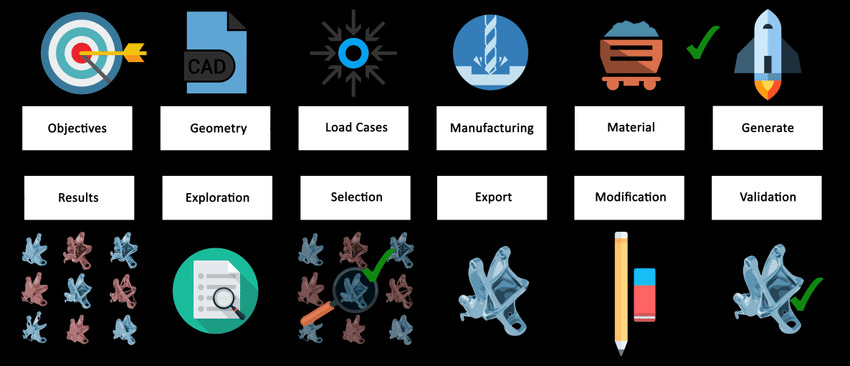
\includegraphics[width=\textwidth]{./images/Autodesk-Generative-Design-Framework.jpeg}
    \end{minipage}
    \caption{Autodesk Prozessablauf}
    \label{fig:meinbild}
  \end{figure}
  
  1.	Ziele: Der Benutzer kann zwischen zwei Optionen wählen, entweder die Masse zu minimieren oder die Steifigkeit zu maximieren. In beiden Fällen wird ein Sicherheitsfaktor benötigt. Bei Auswahl der zweiten Option muss der Anwender auch eine Zielmasse angeben, die die Optimierung erreichen soll.
  2.	Geometrie: Der Benutzer definierte die Bereiche, die von der Optimierung verschont bleiben sollen (Erhaltungsbereiche) und die Bereiche, die leer bleiben müssen (Hindernisbereich). 
  3.	Lastfälle: Generative Design unterstütz Kräfte, Druck und Lagerlast. Es kann auch die Schwerkraft berücksichtigen. Die Lasten müssen auf die vorher erstellten Erhaltungsbereiche angewandt werden. 
  4.	Fertigungsbeschränkungen: Der Benutzer kann Fertigungsbeschränkungen angeben, um die Fertigung später zu erleichtern (5-Achs-Fräsen, 4-Achs-Fräsen). Dies spart Produktionskosten ein.
  5.	Material: Generativ Design ermöglicht die Auswahl von bis zu zehn verschiedenen Materialien in einer Analyse. 
  6.	Eingabeprüfung und Berechnung: Generative Design überprüft, ob alle erforderlichen Informationen korrekt sind. Wenn ja, werden die Optimierungen auf externen Servern durchgeführt. 
  7.	Ergebnisse: Sobald die Ergebnisse auf dem lokalen Computer heruntergeladen sind, können diese Visualisiert werden. 
  8.	Exploration: Generative Design bietet eine dedizierte Umgebung mit Visualiserungswerkzeugen, um die Ergebnisse geordnet darzustellen. Das hilft bei der Identifizierung der besten Lösung.
  9.	Auswahl: Der Anwender wählt die Lösung aus, die am besten den gewünschten Anforderungen entspricht und exportiert diese.
  10.	Export: das Designt wird isoliert und für weitere Änderungen verfügbar gemacht. \ac*{CAD}-Geometrie des Teils wird in die Modellierungsumgebung von Fusion 360 importiert.
  11.	Modifikation: Nach dem Export der Lösung, muss es mit herkömmlichen \ac*{CAD}-Tools bearbeitet werden, um Fehler zu beheben.
  12.	Validierung: Die Leistungsfähigkeit der exportierten Form muss durch zusätzliche Finite-Elemente-Analysen validiert werden. \autocite*{7}

\subsection*{Generatives Design für Leichtgewicht}

Durch das generative Design lässt sich die Materialeffizienz eines Designs verbessern, während die Leistungsparameter und Funktionalitätsanforderungen erhalten bleiben. Die Software entfernt Material an Stellen, an denen es nicht benötigt wird, und strukturiert es organisch um, basierend auf Stress- und Dehnungsmustern. Dadurch kann ein generativ gestaltetes Bauteil bei gleichbleibender Funktionalität eine Materialreduktion von bis zu 80 Prozent erreichen!

\begin{figure}[h]
  \begin{minipage}{0.5\textwidth}
    \centering
    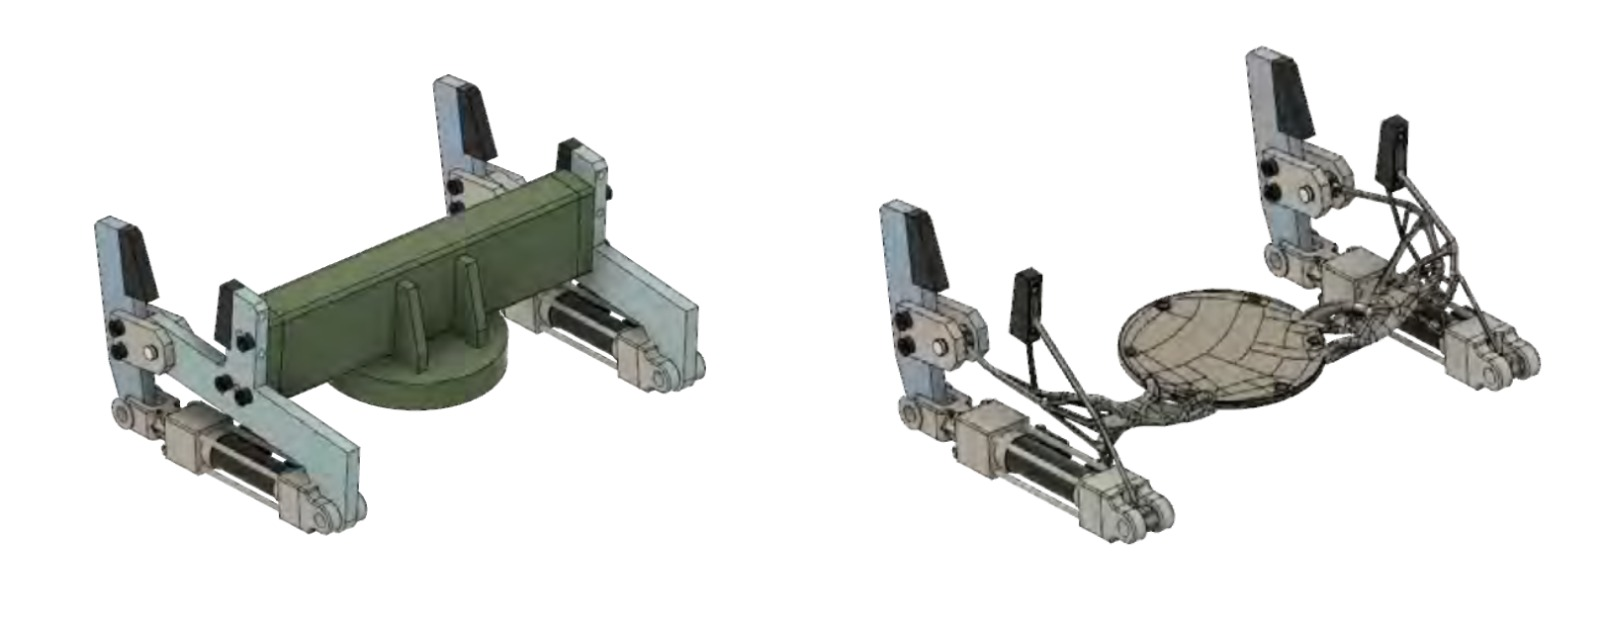
\includegraphics[width=\textwidth]{./images/WhatsApp Image 2023-06-11 at 23.48.25.jpeg}
  \end{minipage}
  \caption{Generativ Designtes Bauteil}
  \label{fig:meinbild}
\end{figure}

Die Herstellung generativ gestalteter Teile erfolgt oft durch additive Fertigung, auch bekannt als 3D-Druck. Additive Fertigung ermöglicht die effiziente Herstellung komplexer Designs, die mit herkömmlichen Verfahren schwer umsetzbar wären. Zwei 3D-Druckverfahren, Powder Bed Fusion (PBF) für Stahl und Fused Deposition Modeling (FDM) für Polycarbonat, sind die am weitesten verbreiteten.

Eine wichtige Komponente des generativen Designs ist die Software Autodesk Netfabb, die Werkzeuge zur Optimierung des 3D-Druck-Workflows bietet. Mit dieser Software können Stützstrukturen, Fütterungs- und Geschwindigkeitseinstellungen optimiert werden, um den Material- und Energieverbrauch zu minimieren.

Um die Umweltauswirkungen der generativ gestalteten Bauteile und des Herstellungsprozesses zu bewerten, wird eine umfassende Lebenszyklusanalyse (LCA) durchgeführt. Diese berücksichtigt den gesamten Lebenszyklus des Bauteils, einschließlich der Rohstoffverarbeitung, der Herstellung, der Nutzung und der Entsorgung. Die Ergebnisse zeigen, dass generativ gestaltete Teile, die mit additiven Verfahren hergestellt werden, eine geringere Umweltbelastung aufweisen als Teile, die mit herkömmlichen Verfahren gefertigt werden.

\subsection*{TestFit Plattform und Fallbeispiel in  Rio de Janeiro}

TestFit ist eine Software für generatives Design im Bauwesen. Sie wurde von der Firma TestFit Inc. entwickelt und bietet eine benutzerfreundliche Oberfläche zur Generierung von Anfangsentwürfen und zur finanziellen Machbarkeitsprüfung von Immobilienprojekten.

Die Software ist in vier Hauptbereiche unterteilt (\autoref{fig:software}). Im oberen linken Bereich können verschiedene Projekte verwaltet und deren Eigenschaften wie städtebauliche Bedingungen, finanzielle Daten, Gebäude- und Einheitenmerkmale angepasst werden. Der untere linke Bereich ermöglicht detaillierte Bearbeitungen wie die Änderung der Gebäudehöhe oder der allgemeinen Gebäudekonfiguration.

Der große obere rechte Bereich der Software bietet verschiedene grafische Ressourcen wie 3D-Visualisierungen und 2D-Pläne, um die generierten Entwürfe zu visualisieren. Der untere rechte Bereich zeigt die generierten Lösungen an, wie die Anzahl der Einheiten pro Fläche und die finanziellen Ergebnisse des Projekts. Es können auch Vergleiche zwischen verschiedenen Entwurfsalternativen durchgeführt werden.

TestFit zeichnet sich durch seine generative Fähigkeit aus, mit der es anhand vorgegebener Parameter optimale Lösungen generiert. Es ermöglicht die Manipulation einer Vielzahl von Baumerkmalen und bietet eine schnelle Algorithmusgenerierung. Die Software unterstützt auch die Erstellung, Bearbeitung und den Vergleich von verschiedenen Entwurfsalternativen.

\begin{figure}[h]
  \begin{minipage}{0.5\textwidth}
    \centering
    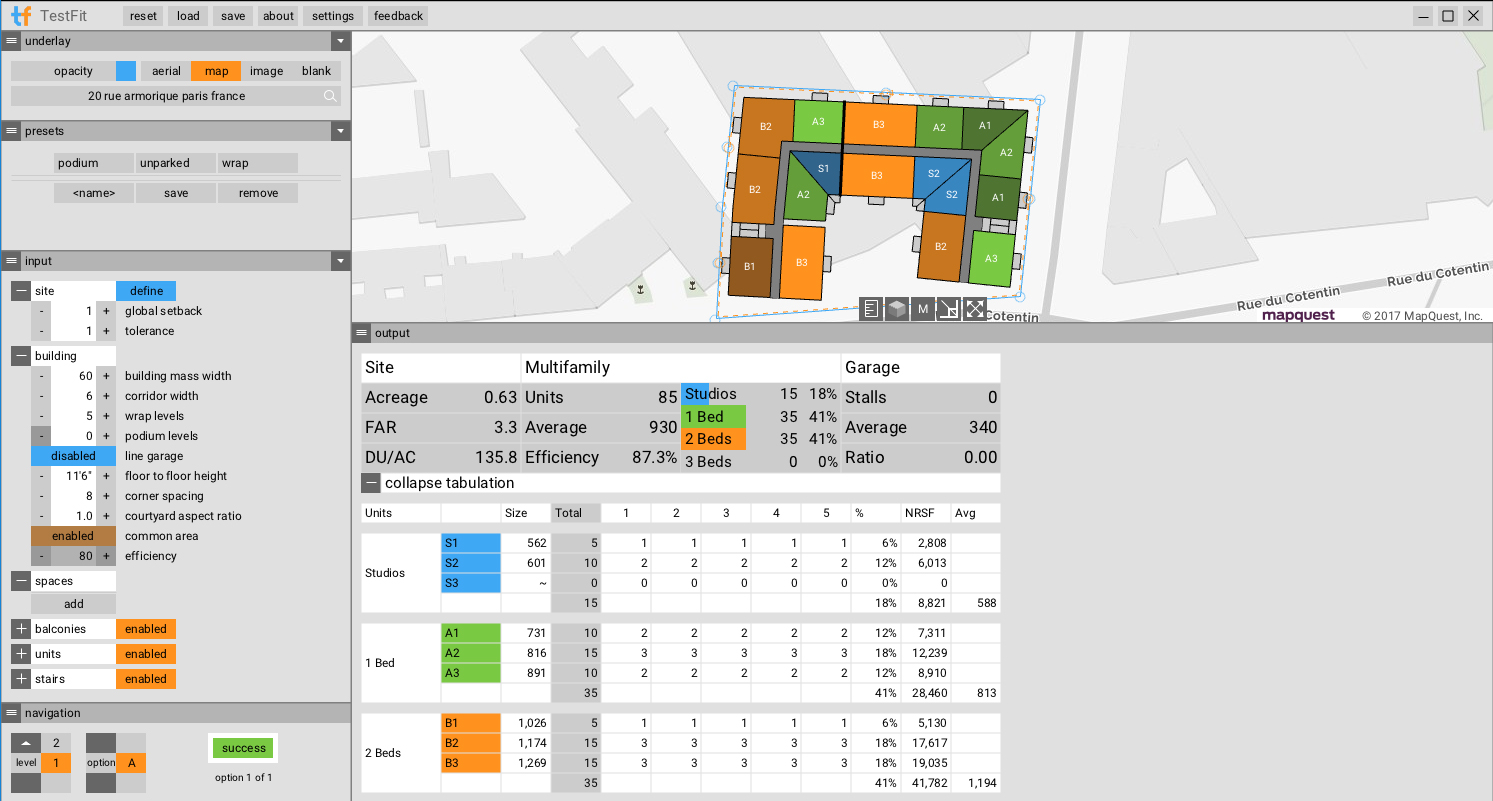
\includegraphics[width=\textwidth]{./images/UnitsData.jpg}
  \end{minipage}
  \caption{TestFit Software}
  \label{fig:software}
\end{figure}

Fallstudie in Rio de Janeiro, bei der das generative Design zur Optimierung der Raumplanung und des Wohnungsbaus eingesetzt wurde. Das Ziel war es, mithilfe einer speziellen Software maximale Raumnutzung und eine vorgegebene Anzahl von Wohnungen mit bestimmten Größen und Anteilen zu erreichen.

Zunächst wurden bestimmte Kriterien definiert, um einen geeigneten Standort in Rio de Janeiro auszuwählen. Es wurde ein Bereich im Stadtteil Santo Cristo identifiziert, der die erforderlichen Voraussetzungen erfüllte, wie ausreichende Größe und bekannte Zonierungsbeschränkungen. Dieser Bereich wurde als "besonderes Gebiet von städtischem Interesse" eingestuft und bot steuerliche Vorteile für den Wohnungsbau.

Die generative Design-Software wurde verwendet, um Lösungen für den Wohnungsbau in diesem Gebiet zu generieren. Die Software ermöglichte die Eingabe verschiedener Parameter wie Gebäudehöhe, Gebäudekonfiguration, Flächennutzung und Wohnungsgrößen. Anhand dieser Parameter generierte die Software automatisch verschiedene Lösungsalternativen.

Zur Bewertung der generierten Lösungen wurden neun Parameter festgelegt, darunter die Gesamtbaufläche, die Anzahl der Einheiten, die durchschnittliche Wohnungsgröße und die Flächenproportionen der verschiedenen Wohnungstypen. Die Ergebnisse wurden analysiert, um festzustellen, inwieweit die Ziele der Maximierung der Raumnutzung und der Generierung der gewünschten Wohnungsanzahl und -größen erreicht wurden.

Es wurden mehrere Iterationen des generativen Designprozesses durchgeführt, um die Lösungen kontinuierlich zu verbessern. Dabei wurden verschiedene Gebäudekonfigurationen und -layouts ausprobiert, um die gewünschten Ergebnisse zu erzielen. \autocite*{17}



\subsection*{Fallbeispiel Heydar Aliyev Centre}
Für das Heydar Aliyev Centre wurde die Software Rhino 3D verwendet. Rhino ist eine 3D-Modellierungssoftware, die sich durch ihre Vielseitigkeit und ihre Fähigkeit zur Generierung komplexer Formen auszeichnet.

\begin{figure}[h]
    \begin{minipage}{0.5\textwidth}
      \centering
      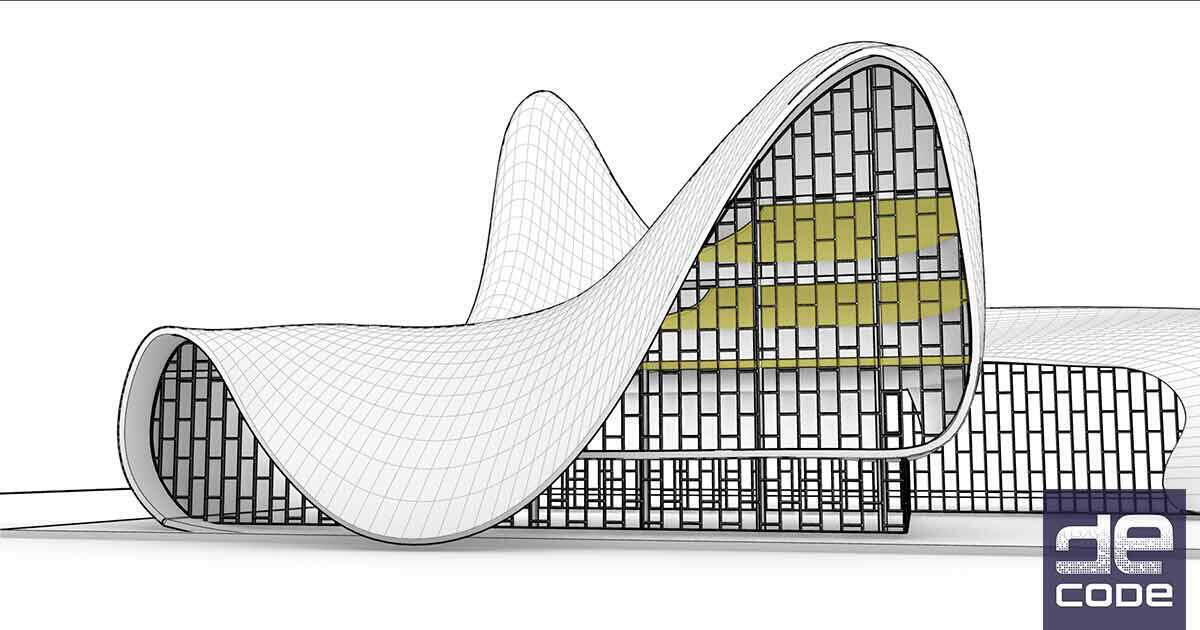
\includegraphics[width=\textwidth]{./images/DE_Rh_lvl1_baku.jpg}
    \end{minipage}
    \caption{Heydar Aliyev Centre}
    \label{fig:centre}
  \end{figure}

Das Heydar Aliyev Centre in Baku, Aserbaidschan ist ein architektonisches Meisterwerk von Zaha Hadid (\autoref{fig:centre}). Es vereint Kunst, Kultur und Geschichte und beeindruckt mit seinen fließenden Formen und der innovativen Raumgestaltung. 
Bei der Gestaltung wurde generatives Design verwendet, um die organischen Kurven und fließenden Formen des Gebäudes zu schaffen. Das Design-Team legte verschiedene Parameter und Kriterien fest wie beispielsweise Raumfunktionen, Nutzungsanforderungen, ästhetische Präferenzen und strukturelle Stabilität. 
Basierend auf diesen Parametern konnte das System unzählige mögliche Designs generieren. Dabei wurden Aspekte wie räumliche Effizienz, natürliche Belichtung, Zugänglichkeit und visuelle Harmonie berücksichtigt. Das generative Design ermöglichte es den Architekten, schnell eine Vielzahl von Variationen zu erforschen und diejenige auszuwählen, die am besten den Anforderungen entsprachen. 
Das Ergebnis ist ein einzigartiges und faszinierende architektonisches Konzept, das ohne den Einsatz von generativem Design vermutlich nicht realisierbar gewesen wäre. Dieses Bauwerk zeigt, wie computergesteuerte Designmethoden neue Horizonte eröffnen. 
Generatives Design hat nicht nur zur Schaffung eines ikonischen Gebäudes beigetragen, sondern es hat auch die Effizienz und Nachhaltigkeit des Designs verbessert. Durch die Berücksichtigung von Faktoren wie Energieeffizienz und optimierte Raumnutzung konnte das Heydar Aliyev Centre eine umweltfreundliche und ressourcenschonende Architektur realisieren. \autocite*{5}


\section{Herausforderungen und Zukunftsaussichten}
\subsection*{Ethische und rechtliche Aspekte}
Im Rahmen des generativen Designs ergeben sich verschiedene ethische und rechtliche Fragestellungen, die in diesem Abschnitt diskutiert werden. Eine der zentralen ethischen Fragen betrifft die Autorenschaft und Originalität generativ gestalteter Werke. Da generatives Design auf Algorithmen und computergenerierten Prozessen basiert, kann die Frage aufgeworfen werden, ob der Designer oder der Algorithmus als Urheber des Kunstwerks oder Designs angesehen werden sollte. Dies wirft Fragen zum geistigen Eigentum und den damit verbundenen Rechten und Verantwortlichkeiten auf.

Ein weiterer ethischer Aspekt betrifft den Einfluss des generativen Designs auf die Arbeitswelt und die Beschäftigung. Die Automatisierung und algorithmische Generierung von Designs könnte traditionelle kreative Berufe beeinflussen und möglicherweise zu Arbeitsplatzverlusten führen. Die ethische Verantwortung besteht darin, die sozialen Auswirkungen solcher Veränderungen zu berücksichtigen und angemessene Lösungen zu finden, um die Arbeitskräfte umzuschulen oder neue Arbeitsbereiche zu schaffen.

Darüber hinaus können Fragen der Privatsphäre und Datensicherheit im Zusammenhang mit generativem Design auftreten. Das Sammeln und Verarbeiten von Daten, um generative Algorithmen zu verbessern, kann bedenklich sein, insbesondere wenn persönliche Daten ohne Zustimmung der betroffenen Personen verwendet werden. Es ist wichtig, Richtlinien und Best Practices zu entwickeln, um den Schutz von persönlichen Informationen und die Einhaltung von Datenschutzgesetzen zu gewährleisten.

Auf der rechtlichen Seite können Fragen zur Haftung und Verantwortung im Falle von Fehlern oder Schäden im Zusammenhang mit generativen Designs auftreten. Wenn ein Algorithmus oder eine KI-gesteuerte Software einen Fehler aufweist, wer trägt dann die Verantwortung? Es ist wichtig, klare rechtliche Rahmenbedingungen zu schaffen, um mögliche Streitigkeiten zu vermeiden und die Haftung angemessen zuzuweisen.

Die Auseinandersetzung mit ethischen und rechtlichen Aspekten des generativen Designs ist von großer Bedeutung, um die potenziellen Auswirkungen dieser Technologie zu verstehen und entsprechende Richtlinien und Regelungen zu entwickeln, um sowohl die Rechte und Interessen der Designer als auch der Gesellschaft als Ganzes zu schützen. Nur durch eine verantwortungsvolle Herangehensweise können die Chancen des generativen Designs genutzt und mögliche Risiken minimiert werden.

\subsection*{Technologische Entwicklung}
Das generative Design ist eng mit technologischen Entwicklungen verbunden, die das Potenzial haben, diese Designpraxis weiter voranzutreiben und zu verbessern. In diesem Abschnitt werden einige relevante technologische Trends und Entwicklungen im Zusammenhang mit generativem Design betrachtet.

1. Fortschritte in der Rechenleistung: Mit dem technologischen Fortschritt und der kontinuierlichen Steigerung der Rechenleistung werden komplexe generative Algorithmen und Simulationen schneller und effizienter. Dies eröffnet neue Möglichkeiten für die Kreation und Optimierung von Designs in Echtzeit und ermöglicht die Verarbeitung großer Datenmengen für noch genauere Ergebnisse.

2. Künstliche Intelligenz (KI): Die Integration von KI-Technologien wie maschinellem Lernen und Deep Learning in den Bereich des generativen Designs eröffnet faszinierende Perspektiven. Durch den Einsatz von KI können generative Algorithmen lernen, Muster zu erkennen, menschliche Präferenzen zu verstehen und aufgrund dieser Erkenntnisse optimierte Designs zu generieren. KI-gesteuerte generative Systeme können kontinuierlich dazulernen und sich anpassen, um den gestalterischen Anforderungen gerecht zu werden.

3. 3D-Druck und additive Fertigung: Der Fortschritt in der 3D-Drucktechnologie ermöglicht es, generativ gestaltete Objekte und Strukturen direkt aus digitalen Modellen herzustellen. Dies eröffnet neue Möglichkeiten für die Umsetzung komplexer und individueller Designs, die mit herkömmlichen Fertigungsmethoden nur schwer realisierbar wären. Generative Designs können speziell auf die Anforderungen des 3D-Drucks abgestimmt werden, um optimale Ergebnisse zu erzielen.

4. Virtual Reality (VR) und Augmented Reality (AR): VR- und AR-Technologien eröffnen neue Wege der Visualisierung und Interaktion mit generativen Designs. Designer können virtuelle Umgebungen nutzen, um ihre Ideen zu visualisieren und zu testen, noch bevor sie physisch umgesetzt werden. AR ermöglicht es, generative Designs in die reale Welt zu projizieren und sie in verschiedenen Kontexten zu betrachten, was wiederum das Designfeedback verbessert und den Entwurfsprozess optimiert.

5. Datenanalyse und -visualisierung: Der Zugang zu großen Datenmengen und die Fortschritte in der Datenanalyse ermöglichen es, generative Designs auf der Grundlage umfangreicher Informationen zu erstellen. Durch die Analyse von Nutzerdaten, Trends und anderen relevanten Informationen können generative Algorithmen personalisierte Designs erzeugen und auf individuelle Präferenzen und Anforderungen reagieren.

Diese technologischen Entwicklungen eröffnen neue Möglichkeiten für das generative Design und werden voraussichtlich zu einer weiteren Integration und Verfeinerung dieser Designpraxis führen. Sie bieten Potenzial für eine verbesserte Kreativität, Effizienz und Innovation in verschiedenen Anwendungsbereichen und werden die Zukunft des generativen Designs maßgeblich beeinflussen.

\subsection*{Potenzial für Innovationen und kreative Lösungen}
Entschuldigung für das Missverständnis. Hier ist der Text zu "Potenzial für Innovationen und kreative Lösungen" als Fließtext:

Generatives Design birgt ein enormes Potenzial für Innovationen und kreative Lösungen in verschiedenen Bereichen. Die Kombination von algorithmischer Intelligenz, Datenanalyse und automatisierter Generierung ermöglicht es Designern, über herkömmliche gestalterische Grenzen hinauszugehen und innovative Ansätze zu entwickeln.

Ein wesentliches Potenzial liegt in der Effizienz- und Optimierungsfähigkeit generativer Designs. Durch die Integration komplexer Parameter und Anforderungen in den Designprozess können Designs optimiert werden. Algorithmen und Simulationen ermöglichen die Ausrichtung auf Effizienz, Festigkeit oder andere Kriterien, was zu besser angepassten und funktionaleren Produkten und Strukturen führt.

Ein weiteres Potenzial liegt in der Personalisierung von Designs. Durch den Einsatz von Datenanalyse und maschinellem Lernen können generative Designansätze personalisierte Designs generieren, die auf individuelle Bedürfnisse und Präferenzen zugeschnitten sind. Kunden können einzigartige Produkte erhalten, die auf spezifische Parameter wie Körpermaße oder individuelle Vorlieben abgestimmt sind. Dies ermöglicht eine maßgeschneiderte Nutzererfahrung und eröffnet neue Möglichkeiten im Bereich des kundenspezifischen Designs.

Generatives Design unterstützt auch die kreative Exploration. Durch den Einsatz von Algorithmen und computerbasierten Modellen können Designer mit einer Vielzahl von Variationen und Möglichkeiten experimentieren. Dies fördert den kreativen Entdeckungsprozess und ermöglicht es, unkonventionelle Ideen zu erforschen und neue ästhetische Ausdrucksformen zu entdecken.

Darüber hinaus bietet generatives Design Potenzial für nachhaltiges Design. Durch die Optimierung von Materialverwendung, Gewichtsreduktion und Energieeffizienz können generative Designs dazu beitragen, Ressourcen zu schonen und ökologische Fußabdrücke zu minimieren. Die Verbindung von generativem Design mit nachhaltigen Materialien und Fertigungsmethoden kann zu innovativen Lösungen im Bereich des umweltbewussten Designs führen.

Ein weiterer Aspekt des Potenzials von generativem Design liegt in der Zusammenarbeit und Co-Creation. Durch den Einsatz von generativen Tools und Plattformen können Designer, Ingenieure und andere Fachleute zusammenarbeiten. Dies fördert den Austausch von Ideen, die Integration unterschiedlicher Fachkenntnisse und die Schaffung interdisziplinärer Lösungsansätze.

Das Potenzial für Innovationen und kreative Lösungen im generativen Design ist weitreichend. Durch den Einsatz von Algorithmen, Datenanalyse und Automatisierung können Designprozesse verbessert und neue Möglichkeiten für die Gestaltung der Zukunft geschaffen werden. Generatives Design ermöglicht effiziente und personalisierte Gestaltung, fördert nachhaltiges Denken und eröffnet Wege für verbesserte Zusammenarbeit und Co-Creation zwischen verschiedenen Fachbereichen.


\section{Fazit}
\subsection*{Vor- und Nachteile}
 Vorteile:

 Effizienzsteigerung: Generatives Design ermöglicht eine schnellere Erstellung und Optimierung von Designs durch automatisierte Prozesse und Algorithmen.
 Individualisierung: Durch die Anpassung an spezifische Parameter und Anforderungen können generative Designlösungen personalisierte und maßgeschneiderte Ergebnisse liefern.
 Innovationspotenzial: Generatives Design eröffnet neue Möglichkeiten für kreative Lösungen und ermöglicht die Exploration unkonventioneller Ideen und ästhetischer Ausdrucksformen.
 Nachhaltigkeit: Durch die Optimierung von Material- und Ressourceneinsatz sowie die Gewichtsreduzierung und Energieeffizienz kann generatives Design zu umweltfreundlicheren Produkten und Strukturen beitragen.
 Zusammenarbeit: Generatives Design fördert die Zusammenarbeit zwischen Designern, Ingenieuren und anderen Fachleuten durch den Einsatz von kreativen Tools und Plattformen. \autocite{12} \autocite*{13}
 Nachteile:
 
 Verlust traditioneller Arbeitsfelder: Die Automatisierung von Designprozessen kann zur Reduzierung oder zum Wegfall von Arbeitsplätzen in bestimmten Bereichen führen.
 Ethische Fragen: Generatives Design wirft Fragen hinsichtlich der Urheberschaft, des geistigen Eigentums und der Verantwortung auf, da die Beteiligung von Algorithmen und computergenerierten Prozessen den kreativen Schöpfungsprozess beeinflusst.
 Komplexität: Die Anwendung generativer Designmethoden erfordert spezifisches technisches Wissen und Fähigkeiten, um komplexe Algorithmen und Tools zu verstehen und zu nutzen.
 Abhängigkeit von Daten: Generatives Design basiert auf der Verarbeitung großer Datenmengen. Der Zugriff auf relevante und qualitativ hochwertige Daten kann eine Herausforderung darstellen.
 Technologische Einschränkungen: Die effektive Anwendung generativer Designmethoden kann von den verfügbaren technologischen Ressourcen, wie Rechenleistung und Software, abhängen. \autocite*{13}

\subsection*{Beantwortung der Forschungsfrage}

Forschungsfrage „Wie unterstützt generatives Design die Gestaltungsprozesse?“ 

Generatives Design unterstützt die Gestaltungsprozesse auf vielfältige Weise. Es bietet Designerinnen und Designern innovative Werkzeuge und Techniken, um kreative Lösungen zu entwickeln und komplexe Designherausforderungen zu bewältigen.

Exploration und Ideengenerierung: Generatives Design ermöglicht es Designern, mit einer Vielzahl von Variationen und Möglichkeiten zu experimentieren. Durch den Einsatz von Algorithmen und computergestützten Modellen können Designer alternative Designs und Lösungsansätze erkunden, die sie möglicherweise nicht eigenständig entwickelt hätten. Dies fördert die kreative Exploration und unterstützt den Ideengenerierungsprozess.

Optimierung und Effizienz: Generatives Design integriert komplexe Parameter und Anforderungen in den Designprozess, um optimierte Ergebnisse zu erzielen. Algorithmen und Simulationen ermöglichen die Anpassung von verschiedenen Designkriterien wie Festigkeit, Effizienz oder Materialverbrauch. Durch die automatische Generierung und Bewertung verschiedener Designoptionen können Designer effizientere und funktionalere Lösungen entwickeln.

Personalisierung und Individualisierung: Generatives Design basiert oft auf Datenanalyse und maschinellem Lernen, um personalisierte Designs zu erstellen. Durch die Integration von Benutzerdaten und Präferenzen können generative Algorithmen individuelle Anforderungen und Vorlieben berücksichtigen. Dies ermöglicht die Erstellung maßgeschneiderter Designs, die spezifisch auf die Bedürfnisse und Wünsche der Nutzer zugeschnitten sind.

Schnelle Prototypenerstellung: Generatives Design ermöglicht eine schnellere Erstellung von Prototypen und Iterationen. Durch den Einsatz von 3D-Druck und anderen Rapid-Prototyping-Technologien können generative Designlösungen schnell in physische Modelle umgesetzt werden. Dies beschleunigt den Designprozess und ermöglicht eine frühzeitige Überprüfung und Validierung der entworfenen Lösungen.

Interdisziplinäre Zusammenarbeit: Generatives Design fördert die Zusammenarbeit und Kooperation zwischen verschiedenen Fachbereichen. Durch die Nutzung von kollaborativen Tools und Plattformen können Designer, Ingenieure und andere Experten gemeinsam an einem Designprojekt arbeiten. Dies ermöglicht den Austausch von Wissen und Perspektiven, die Integration unterschiedlicher Expertisen und die Schaffung interdisziplinärer Lösungen.

 \subsection*{Kritische Bewertung und Ausblick}

Zweifellos hat generatives Design  viele Vorteile und Möglichkeiten, aber es gibt auch einige kritische Aspekte, die berücksichtigt werden müssen. Die kritische Bewertung des Reproduktionsdesigns ermöglicht die Identifizierung von Herausforderungen und potenziellen Einschränkungen sowie eine realistische Vision der zukünftigen Entwicklung. 
 Eine der Herausforderungen ist die Komplexität generativer Designmethoden und -algorithmen. Für den effektiven Einsatz und die Erzielung der gewünschten Ergebnisse ist ein gewisses Maß an technischem Wissen und Erfahrung erforderlich. Es besteht die Gefahr, dass Designer von der Technologie abhängig werden und  kreative Intuition und Designfähigkeiten vernachlässigen.  Ein weiteres kritisches Thema ist der Datenschutz und die ethische Nutzung von Informationen im Reproduktionsdesign. Für die Erstellung individueller Modelle sind häufig umfangreiche Benutzerinformationen erforderlich. Es ist wichtig sicherzustellen, dass die Datenschutzbestimmungen befolgt werden und die Privatsphäre der Benutzer respektiert wird. Darüber hinaus sollten mögliche Voreingenommenheit und Diskriminierung, die sich aus der Verwendung der Daten ergeben können, vermieden werden. 
 Darüber hinaus können automatisierte generative Designprozesse die menschliche Kreativität und Originalität beeinflussen. Es besteht die Gefahr, dass reproduktive Designs stereotyp oder repetitiv werden und die einzigartige künstlerische Vision des Designers verloren geht. Die Herausforderung besteht darin, einen geeigneten Gleichgewichtspunkt zu finden, bei dem generatives Design  Unterstützung und Inspiration bietet, menschliche Kreativität und Intuition jedoch im Mittelpunkt stehen. 
 Die Zukunft des reproduktiven Designs zeigt, dass sich die Technologie weiterentwickeln wird. Die Entwicklung effizienterer Algorithmen, fortschrittlicher künstlicher Intelligenz und maschinellem Lernen erweitert die Möglichkeiten des generativen Designs. Dies könnte zu einer breiteren Anwendung in verschiedenen Branchen führen, darunter Robotikdesign, Smart Cities, Virtual Reality und viele andere. Es ist auch zu erwarten, dass die Mensch-Maschine-Interaktion im generativen Design zunehmen wird. Die Kombination aus menschlicher Kreativität und maschineller Intelligenz kann zu einer Synergie führen, die zu noch innovativeren und attraktiveren Designs führt. Die Zusammenarbeit zwischen Designern und Algorithmen wird wahrscheinlich weiter zunehmen und neue Formen des kollaborativen Designs ermöglichen. 
 Zusammenfassend lässt sich sagen, dass generatives Design ein spannendes und vielversprechendes Feld ist, das die Designbranche nachhaltig beeinflussen wird. Es bietet vielfältige Möglichkeiten, Herausforderungen zu bewältigen und innovative Projektlösungen zu entwickeln. Es ist jedoch wichtig, kritische Aspekte zu berücksichtigen, um eine ausgewogene Anwendung des reproduktiven Designs sicherzustellen. Zusammen mit dem Fortschritt 
 
  Technologie und Kreativität erwartet uns ein spannender Blick in die Zukunft des generativen Designs.


\listoffigures
\addcontentsline{toc}{section}{Abbildungsverzeichniss}

\section*{Abkürzungsverzeichnis}
\begin{acronym}
  \acro{ki}[KI]{Künstliche Intelligenz}
  \acro{gd}[GD]{Generatives Design }
  \acro{gD}[gD]{generativen Designs}
  \acro{GAN}[GAN]{Generative Adversarial Network}
  \acro{GAN}[GANs]{Generative Adversarial Networks}
  \acro{CAD}[CAD]{computer aided design}

\end{acronym}

\section*{Literaturverzeichnis}
\printbibliography[heading=none]{}

\end{document}
